\documentclass{book}
\usepackage[utf8]{inputenc}
\usepackage[T1]{fontenc}
%\usepackage[ngerman]{babel}
\usepackage{graphicx}
\usepackage{geometry}
\usepackage{tikz}
\usetikzlibrary{circuits.logic.US, positioning}
\geometry{margin=25mm}

\newcommand{\AuthorName}{Leonard Röpcke}
%\newcommand{\Institute}{Zepellin Gewerbeschule Konstanz}
\newcommand{\Subtitle}{In diesem Buch wird die Transistor Logik so weit abstahiert, dass es möglich ist selber mit Transistoren einen Computer zu bauen.}
\newcommand{\MyDate}{\today}

\begin{document}
\begin{titlepage}
  \centering
  {\scshape\LARGE \par}
  \vspace{2.5cm}
  {\huge\bfseries Von 0 und 1 zu einem Computer\par}
  \vspace{0.8cm}
  {\Large\itshape \Subtitle \par}
  \vfill
  {\Large Autor\par}
  {\Large \AuthorName \par}
  \vspace{1cm}
  {\Large Datum\par}
  {\Large \MyDate \par}
  \vfill
  % Optional: Bild einfügen (Datei hinzufügen oder Zeile auskommentieren)
  % \includegraphics[width=6cm]{example-image}
  \vspace{1cm}
  {\small }
  %unten am anfang
\end{titlepage}
\tableofcontents
\newpage

\mainmatter
\chapter{Einleitung}
\section{Forwort}
Guten Tag, mein Name ist Leonard Röpcke und all das wissen das ich in diesem Buch weitergebe habe ich mir selber angeeignet. 
Weshalb sie immer ein bisschen skeptisch sein sollten und ruig etwas hinterfragen sollten.


\section{Grundlagen der digitalen Logik}
test 



%\begin{tikzpicture}[circuit logic US, scale=1, every node/.style={transform shape}]
    % Eingänge
    %\node (A) at (0,1) [label=left:A] {};
    %\node (B) at (0,-1) [label=left:B] {};

    % AND Gatter
    %\node (and) [and gate, draw, right=of nota, yshift=0cm, xshift=1cm] {};
    
    %Nand
    %\node (nand) [nand gate, draw, right=of notb, yshift=0.75cm] {};

    % OR Gatter (XOR Ausgang)
    %\node (or) [or gate, draw, right=of and, xshift=-0.75cm, yshift=-0.75cm] {};

    % Verbindungen
    %\draw (A.east) -- ++(0.5,0) |- (nota.input);
    %\draw (B.east) -- ++(0.5,0) |- (notb.input);

    %\draw (nota.output) -- (and1.input 1);
    %\draw (B.east) -- ++(1,0) |- (and1.input 2);

    %\draw (A.east) -- ++(1,0) |- (and2.input 1);
    %\draw (notb.output) -- (and2.input 2);

    %\draw (and1.output) -- ++(1,0) |- (or1.input 1);
    %\draw (and2.output) -- ++(1,0) |- (or1.input 2);

    % Ausgang
    %\node[right=of or1.output, label=right:Ausgang] {};
    %\draw (or1.output) -- ++(1,0);

%\end{tikzpicture}


\begin{figure}[h]
  \centering
  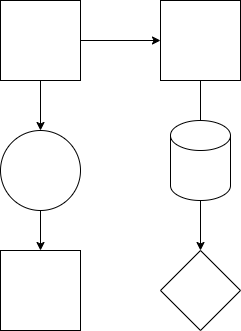
\includegraphics[width=0.5\textwidth]{diagram.png}
  \caption{Test Diagramm mit draw.io erstellt}
  \label{fig:diagram}
\end{figure}


\end{document}